


\subsection{Initial boundary problem}

\begin{frame}{An initial boundary problem}

 \begin{block}{Definition on a semi-infinite strip}
Dane:
\begin{itemize}    
\item $a>0$
\item $g_1(t), g_2(t); t \ge 0$
\item $f_1(x), 0 \le x\le a$
\item $f_2(x), 0 < x < a$
\end{itemize}
	
\end{block}

\end{frame}

\begin{frame}
  \centerline{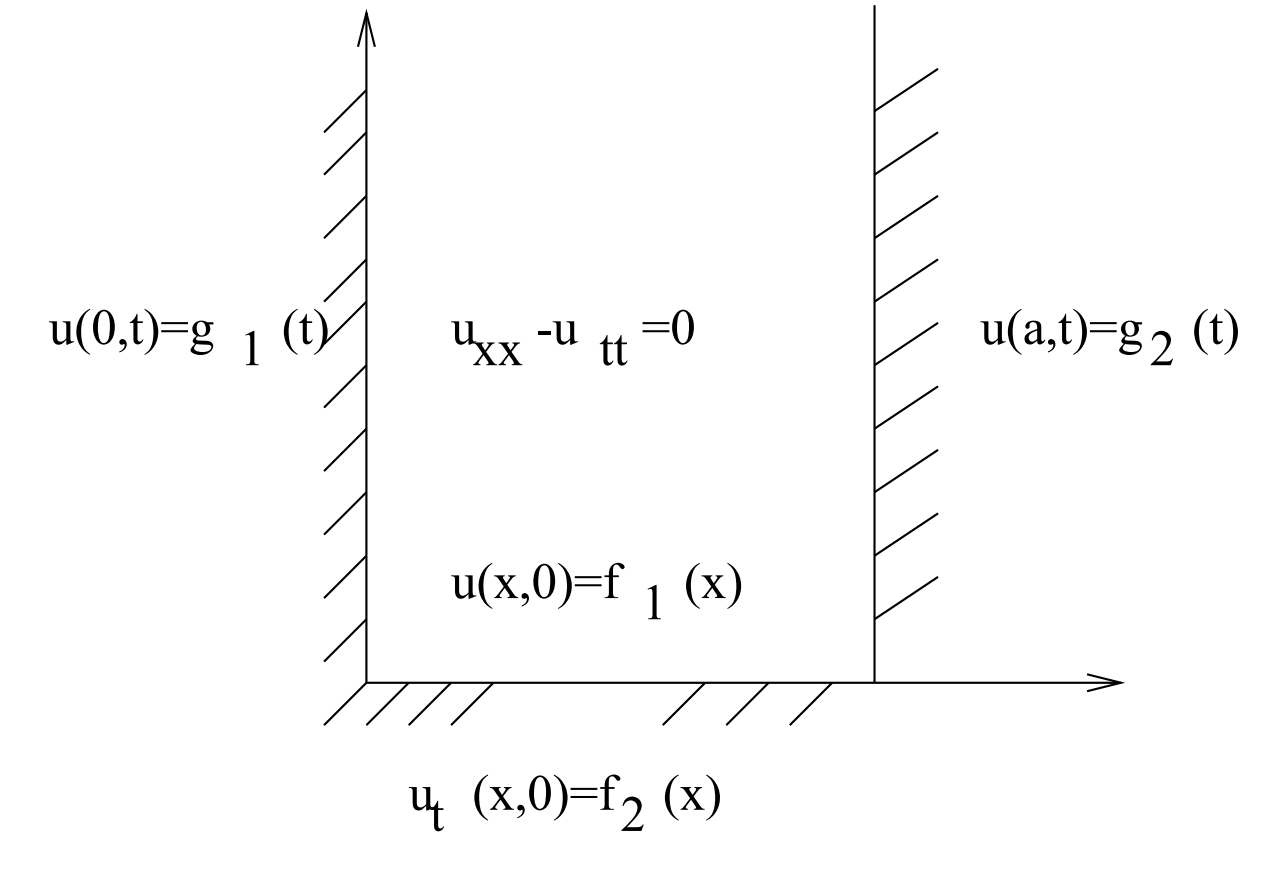
\includegraphics[height = 0.85 \textheight]{img/23/initial_boundary}}
\end{frame}

\begin{frame}
  Szukana funkcja u(x,t), ciągła dla $0 < x < a, t > 0$
spełnia warunki początkowy i brzegowy:

\begin{subnumcases}{\text{initial condition}}
 u(x,0) = f_1(x), 0 \ge x \ge a \label{first} \\
 u_t(x,0) = f_2(x), 0 < x < a \label{second}
\end{subnumcases}

\begin{subnumcases}{\text{boundary condition}}
 u(0,t) = g_1(t), t\ge 0  \\
u(a,t) = g_2(t), t \ge 0
\end{subnumcases}


  \begin{block}{Rozwiązania}
Cauchy-problem $\to$ wzór D'Alemberta \\
initial boundary problem $\to$ szereg Fouriera
 
  \end{block}
\begin{alertblock}{Ale...}
\begin{itemize}
\item nie gdy nieliniowe
\item trudności z wyznaczeniem
\end{itemize}
\end{alertblock}
\end{frame}
